% VLDB template version of 2020-03-05 enhances the ACM template, version 1.7.0:
% https://www.acm.org/publications/proceedings-template
% The ACM Latex guide provides further information about the ACM template

\documentclass{article}
\usepackage{listings}
\usepackage[margin=20mm]{geometry}
\usepackage{graphicx}
\usepackage{amsfonts}
\usepackage{amsmath}
\usepackage{physics}
\usepackage{parskip}
\usepackage{enumitem}
\usepackage{cancel}

%% The following content must be adapted for the final version
% paper-specific
\newcommand\vldbdoi{XX.XX/XXX.XX}
\newcommand\vldbpages{XXX-XXX}
% issue-specific
\newcommand\vldbvolume{14}
\newcommand\vldbissue{1}
\newcommand\vldbyear{2020}
% should be fine as it is
\newcommand\vldbauthors{\authors}
\newcommand\vldbtitle{\shorttitle} 
% leave empty if no availability url should be set
\newcommand\vldbavailabilityurl{http://vldb.org/pvldb/format_vol14.html}

\newtheorem{theorem}{Teor.}
\newtheorem{definition}{Def.}
\newtheorem{example}{Ej.}
\newtheorem{excercise}{Ejer.}

\begin{document}

\textbf{For myself:}

\begin{align}
	\mathrm E_{Y|X}\left(Y-c\right)^2&=\mathrm E_{Y|X}\left(Y^2-2cY+c^2\right)\\
	&=\mathrm E_{Y|X}Y^2-2c\,\mathrm E_{Y|X}Y+c^2\\
	&=\left[\mathrm E_{Y|X}Y^2-\left(\mathrm E_{Y|X}Y\right)^2\right]+\left(\mathrm E_{Y|X}Y-c\right)^2,
\end{align}
whence it follows that
\begin{align}
	\arg\min\mathrm E_{Y|X}\left(Y-c\right)^2&=\mathrm E_{Y|X}Y,\\
	\min\mathrm E_{Y|X}\left(Y-c\right)^2&=\mathrm E_{Y|X}Y^2-\left(\mathrm E_{Y|X}Y\right)^2\\
	&=\mathrm{Var}(Y|X).
\end{align}

\textbf{Ex. 2.1: }Suppose each of $K$-classes has an associated target $t_k$, which is a vector of all zeros, except a one in the $k$th position. Show that classifying to the largest element of $\hat{y}$ amounts to choosing the closest target, $\min_k\norm{t_k-\hat{y}}$, if the elements of $\hat{y}$ sum to one.

\textbf{Answer:}

Let $\hat{y}\in\mathbb R^p:\,\sum_i\hat{y}_i=1$. Then, for any $j$,
\begin{align}
	\norm{t_j-\hat{y}}^2&=\sum_{i\neq j}\hat{y}_i^2+\left(1-\hat{y}_j\right)^2\\
	&=\sum_{i\neq j}\hat{y}_i^2+\left(\sum_{i\neq j}\hat{y}_i\right)^2\\
	&=2\sum_{h,i\neq j;h\leq i}\hat{y}_h\hat{y}_i\\
	&=2\sum_{h\leq i}\hat{y}_h\hat{y}_i-2\sum_{h=j\vee i=j,h\leq i}\hat{y}_h\hat{y}_i\\
	&=2\sum_{h\leq i}\hat{y}_h\hat{y}_i-2\sum_i\hat{y}_k\hat{y}_i\\
	&=2\sum_{h\leq i}\hat{y}_h\hat{y}_i-2\hat{y}_k\sum_i\hat{y}_i\\
	&=2\sum_{h\leq i}\hat{y}_h\hat{y}_i-2\hat{y}_k\\
\end{align}

Soo, if the closest thingy is the $k$th,
\begin{align}
	\norm{t_k-\hat{y}}&\leq\norm{t_j-\hat{y}}\forall j,\\
	\norm{t_k-\hat{y}}^2&\leq\norm{t_j-\hat{y}}^2\forall j,\\
	2\sum_{h\leq i}\hat{y}_h\hat{y}_i-2\hat{y}_k&\leq2\sum_{h\leq i}\hat{y}_h\hat{y}_i-2\hat{y}_j\forall j,\\
	\hat{y}_k&\geq\hat{y}_j\forall j.
\end{align}

\textbf{Ex. 2.2: }Show how to compute the Bayes decision boundary for the simulation example in Figure 2.5.

\textbf{Answer:}

Maybe the previous excercise was meant to help with this one, since we have to pick $k$ such that $p_k\geq p_j\forall j$ with $p$ in the probability simplex, which is equivalent to picking the axis closest to $p$. But that doesn't look less computationaly expensive. In the general case, I guess you could construct a grid and simply check for those conditions.

In the case of a binary classification problem, you can take advantage in the fact that the decision boundary takes the form $p_1=0.5$, and just move along the unique choice perpendicular to the gradient of $p_1$.

\textbf{Ex. 2.3: }Derive equation (2.24).

\textbf{Answer:}

We have a uniform probability distribution along $S_p=\{x\in\mathbb R^p:\,\norm{x}\leq1\}$, and we take $N$ samples. The median minimum distance is such that the probability of a smaller minimum distance be $1/2$. The probability that the minimum distance is above $r$ is the probability that all $N$ samples are above $r$, which should be the $N$th power of the probability that any individual sample is above $r$, which is $1-r^p$. That is,
\begin{align}
	P(\norm{x}\geq r)&=\left(1-r^p\right)^N
\end{align}
and, setting this to equal 1/2, we get
\begin{align}
	d(p,\,N)&=\left(1-\frac{1}{2^{1/N}}\right)^{1/p}.
\end{align}

Thank God for commulative probabilities.

\textbf{Ex. 2.4: }The edge effect problem discussed on page 15 is not peculiar to uniform sampling from bounded domains. Consider inputs drawn from a spherical multinormal distribution $X\sim N(0,\,\mathbf I_p)$. The squared distance from any sample point to the origin has a $\chi^2_p$ distribution with mean $p$. Consider a prediction point $x_0$ drawn from this distribution, and let $a=x_0/\norm{x_0}$ be an associated unit vector. Let $z_i=a^{\mathrm T}x_i$ be the projection of each of the training points in this direction.
\begin{enumerate}[label=\alph*]
	\item Show that the $z_i$ are distributed $N(0,\,1)$ with expected squared distance from the origin 1, while the target point has expected squared distance $p$ from the origin.
	\item For $p=10$ show that the expected distance of a test point from the center of the training data is $3.1$ standard deviations, while all the training points have expected distance $1$ along direction $a$. So most prediction points see themselves as lying on the edge of the training set.
\end{enumerate}

\textbf{Answer:}

\textbf{Part a:}

$N(0,\,\mathbf I_p)$ is precisely obtained as the probability distribution of a point each of whose components are taken from $N(0,\,1)$, which shows $a^Tx_i$ is taken from a distribution $N(0,\,1)$.

Long road: Let $P_X=N(\mu,\,\Sigma)$, which is to say
\begin{align}
	P_X(x)&=\frac{1}{\sqrt{2\pi\det\Sigma}^p}\exp\left(-\frac12\left(x-\mu\right)^T\Sigma^{-1}\left(x-\mu\right)\right).
\end{align}
Then,
\begin{align}
	P_{a^TX}(y)&=\int_{\mathbb R^p}\mathrm dx\,P_X(x)\delta(a^Tx-y)\\
	&=\int_{\mathbb R^p:\,a^Tx=y}\mathrm dx\,P_X(x)\frac{1}{\cancelto{1}{\norm{a}}}.
\end{align}
We now take into account that $a^Tx=y$ means $x=\sum_ix_iu_i+ya=x_\perp+ya$ for $\{a, u_i\}$ an orthonormal basis. This way, and decomposing $\mu=\mu_\perp+\mu_aa$,
\begin{align}
	(x-\mu)^T\Sigma^{-1}(x-\mu)&=(x_\perp-\mu_\perp+(y-\mu_a)a)^T\Sigma^{-1}(x_\perp-\mu_\perp+(y-\mu_a)a)\\
	&=(x_\perp-\mu_\perp)^T\Sigma^{-1}(x_\perp-\mu_\perp)\\
	&+2(x_\perp-\mu_\perp)^T\Sigma^{-1}(y-\mu_a)a\\
	&+(y-\mu_a)^2a^T\Sigma^{-1}a.
\end{align}
Aaand so we plug all that into the big integral. The (exponential of the) last term can be taken outside the integral, whereas the other two represent stuff to integrate. The contributions from $x_\perp-\mu_\perp$ and $\mu_\perp-x_\perp$ cancel out the second factor, and so it ends up being a constant factor. We can then conclude the probability distribution for $y$ is $N(\mu_a,\,a^T\Sigma^{-1}a)$.

On the other hand, the expected square distance $\mathrm E\norm{x}^2$ is given by
\begin{align}
	\mathrm E\norm{x}^2&=\frac{\int\mathrm dx\,\norm{x}^2\exp\left(-\frac12\norm{x}^2\right)}{\int\mathrm dx\,\exp\left(-\frac12\norm{x}^2\right)}\\
	&=\frac{\int_0^\infty\mathrm dr\,r^{p-1}\int\mathrm d\Theta\,r^2\exp\left(-\frac12r^2\right)}{\int_0^\infty\mathrm dr\,r^{p-1}\int\mathrm d\Theta\,\exp\left(-\frac12r^2\right)}\\
	&=\frac{\int_0^\infty\mathrm dr\,r^{p+1}\exp\left(-\frac12r^2\right)}{\int_0^\infty\mathrm dr\,r^{p-1}\exp\left(-\frac12r^2\right)}\\
	&=\frac{\int_0^\infty\mathrm d\left(\frac12r^2\right)\,2^{\frac12p}\left(\frac12r^2\right)^{\frac12p}\exp\left(-\frac12r^2\right)}{\int_0^\infty\mathrm d\left(\frac12r^2\right)\,2^{\frac12p-1}\left(\frac12r^2\right)^{\frac12p-1}\exp\left(-\frac12r^2\right)}\\
	&=2\frac{\int_0^\infty\mathrm dt\,t^{\frac12p}\exp(-t)}{\int_0^\infty\mathrm dt\,t^{\frac12p-1}\exp(-t)}\\
	&=2\frac{\Gamma\left(\frac12p+1\right)}{\Gamma\left(\frac12p\right)}\\
	&=p.
\end{align}

Note to self: Gamma thingy can be done through parts:
\begin{align}
	\Gamma(x+1)&=\int_0^\infty\mathrm dt\,t^x\exp(-t)\\
	&=\cancelto{0}{\left[-xt^{x-1}\exp(-t)\right]_0^\infty}+\int_0^\infty\mathrm dt\,xt^{x-1}\exp(-t)\\
	&=x\Gamma(x)
\end{align}

\textbf{Part b:}

If we compute the expected distance as $\sqrt{\mathrm E\norm{x}^2}$ we're left with about $3.16$, which I guess is what the author did. And here I was, about to compute $\mathrm E\norm{x}$. In fact, let's do it for the lulz.

\begin{align}
	\mathrm E\norm{x}&=\frac{\int\mathrm dr\,\norm{x}\exp\left(-\frac12\norm{x}^2\right)}{\int\mathrm dx\,\exp\left(-\frac12\norm{x}^2\right)}\\
	&=\cdots\\
	&=\frac{\int\mathrm dr\,r^p\exp\left(-\frac12r^2\right)}{\int\mathrm dx\,r^{p-1}\exp\left(-\frac12r^2\right)}\\
	&=\sqrt{2}\frac{\Gamma\left(\frac12p+\frac12\right)}{\Gamma\left(\frac12p\right)}\\
	&\approx3.08.
\end{align}

For the expected distance along direction $a$, we get $1$ as the square root of the expected square distance, and
\begin{align}
	\mathrm E\norm{x}&=\frac{\int_0^\infty\mathrm dr\,r\exp\left(-\frac12r^2\right)}{\int_0^\infty\mathrm dr\,\exp\left(-\frac12r^2\right)}\\
	&=\frac{\int_0^\infty\mathrm dt\,\exp(-t)}{\sqrt{\frac\pi2}}\\
	&=\frac2\pi\\
	&\approx0.78.
\end{align}

\textbf{Ex. 2.5: }

\begin{enumerate}[label=\alph*]
	\item Derive equation (2.27). The last line makes use of (3.8) through a conditioning argument.
	\item Derive equation (2.28), making use of the \textit{cyclic} property of the trace operator $[\Tr(AB)=\Tr(BA)]$, and its linearity (which allows to interchange the order of trace and expectation).
\end{enumerate}

\textbf{Answer:}

The relationship between the random variables $X$ and $Y$ is
\begin{align}
	Y=X^T\beta+\varepsilon,
\end{align}
with $\varepsilon\sim N(0,\,\sigma)$ and $X$ taking values in $\mathbb R^p$. As a training set, we have $N$ inputs arranged in row form into matrix $\mathbf X\in\mathbb R^{N\times p}$, and $N$ outputs aranged in $\mathbf y\in\mathbb R^{N\times1}$ of the form $\mathbf y=\mathbf X\beta+\pmb\varepsilon$, where $\pmb\varepsilon$ is a vector of samples from $\varepsilon$'s probability distribution function.

So, the expected prediction error at input value $x_0$ is given by
\begin{align}
	\mathrm{EPE}(x_0)&=\mathrm E_{y_0|x_0}\mathrm E_{\mathcal T}\left(y_0-\hat{y_0}\right)^2,\\
	\mathrm E_{y_0|x_0}&=\int\mathrm dy_0\,P(y_0|x_0),\\
	\mathrm E_{\mathcal T}&=\mathrm E_{\mathbf X}\mathrm E_{\varepsilon}\\
	&=\int\mathrm d\mathbf X\,P(\mathbf X)\int\mathrm d\pmb\varepsilon\,P(\pmb\varepsilon).
\end{align}

We observe that all $y_0$ ($\varepsilon$), $\mathbf X$ and $\pmb\varepsilon$ are independent variables, whence the expectation values commute.

The estimated value is defined by
\begin{align}
	\hat{y_0}&=x_0^T\hat{\beta},\\
	\hat{\beta}&=(\mathbf X^T\mathbf X)^{-1}\mathbf X^T\mathbf y\\
	&=(\mathbf X^T\mathbf X)^{-1}\mathbf X^T\left(\mathbf X\beta+\pmb\varepsilon\right)\\
	&=\beta+\left(\mathbf X^T\mathbf X\right)^{-1}\mathbf X^T\pmb\varepsilon.
\end{align}

We thus have:
\begin{align}
	\mathrm E_{y_0|x_0}y_0&=\mathrm E_{\varepsilon|x_0}\left(x_0^T\beta+\varepsilon\right)\\
	&=x_0^T\beta+\cancelto{0}{\mathrm E_{\varepsilon|x_0}\varepsilon},\\
	\mathrm{Var}(y_0|x_0)&=\mathrm E_{\varepsilon|x_0}\left(y_0-\mathrm E_{\varepsilon|x_0}y_0\right)^2\\
	&=\mathrm E_{\varepsilon|x_0}\left(x_0^T\beta+\varepsilon-x_0^T\beta\right)^2\\
	&=\mathrm E_{\varepsilon|x_0}\varepsilon^2=1,\\
	\mathrm E_{\mathcal T}\hat{y_0}&=\mathrm E_{\mathcal T}\left(x_0^T\hat{\beta}\right)\\
	&=\mathrm E_{\mathcal T}\left(x_0^T\beta+\varepsilon\right)\\
	&=x_0^T\beta+\cancelto{0}{\mathrm E_{\mathcal T}\varepsilon},\\
	\mathrm{Var}\hat{y_0}&=\mathrm E_{\mathcal T}\left(\hat{y_0}-\mathrm E_{\mathcal T}\hat{y_0}\right)^2\\
	&=\mathrm E_{\mathcal T}\left(x_0^T\beta+x_0^T\left(\mathbf X^T\mathbf X\right)^{-1}\mathbf X^T\pmb\varepsilon-x_0^T\beta\right)^2\\
	&=\mathrm E_{\mathcal T}\left(x_0^T\left(\mathbf X^T\mathbf X\right)^{-1}\mathbf X^T\pmb\varepsilon\right)^2\\
	&=\mathrm E_{\mathcal T}x_0^T\left(\mathbf X^T\mathbf X\right)^{-1}\mathbf X^T\pmb\varepsilon\pmb\varepsilon^T\mathbf X\left(\mathbf X^T\mathbf X\right)^{-1}x_0\\
	&=\mathrm E_{\mathbf X}x_0^T\left(\mathbf X^T\mathbf X\right)^{-1}\mathbf X^T\mathrm E_{\pmb\varepsilon}\left(\pmb\varepsilon\pmb\varepsilon^T\right)\mathbf X\left(\mathbf X^T\mathbf X\right)^{-1}x_0\\
	&=\mathrm E_{\mathbf X}x_0^T\left(\mathbf X^T\mathbf X\right)^{-1}\mathbf X^T\sigma^2\mathrm I_N\mathbf X\left(\mathbf X^T\mathbf X\right)^{-1}x_0\\
	&=\sigma^2\mathrm E_{\mathbf X}x_0^T\left(\mathbf X^T\mathbf X\right)^{-1}x_0\\
\end{align}

Now,
\begin{align}
	\mathrm{EPE}(x_0)&=\mathrm E_{y_0|x_0}\mathrm E_{\mathcal T}\left(y_0-\hat{y_0}\right)^2\\
	&=\mathrm E_{y_0|x_0}y_0^2-2\mathrm E_{y_0|x_0}y_0\mathrm E_{\mathcal T}\hat{y_0}+\mathrm E_{\mathcal T}\hat{y_0}^2\\
	&=\mathrm{Var}(y_0|x_0)+\left(\mathrm E_{y_0|x_0}y_0\right)^2-2\mathrm E_{y_0|x_0}y_0\mathrm E_{\mathcal T}\hat{y_0}+\mathrm{Var}_{\mathcal T}(\hat{y_0})+\left(\mathrm E_{\mathcal T}\hat{y_0}\right)^2\\
	&=\mathrm{Var}(y_0|x_0)+\mathrm{Var}_{\mathcal T}(\hat{y_0})+\left(\mathrm E_{y_0|x_0}y_0-\mathrm E_{\mathcal T}\hat{y_0}\right)^2\\
	&=\mathrm{Var}(y_0|x_0)+\mathrm{Var}_{\mathcal T}(\hat{y_0})+\mathrm{Bias}^2(\hat{y_0})\\
	&=\sigma^2+\sigma^2x_0^T\mathrm E_{\mathbf X}(\mathbf X^T\mathbf X)^{-1}x_0+0.
\end{align}

Since
\begin{align}
	\mathbf X^T\mathbf X=\left(\sum_\mu x_i^\mu x_j^\mu\right),
\end{align}
and assuming $\mathrm EX=0$ for each element, this is approximately $N\mathrm{Cov}(X)$. So,
\begin{align}
	\mathrm E_{x_0}\mathrm{EPE}(x_0)&=\sigma^2+\frac{\sigma^2}{N}\mathrm E_{x_0}\left(x_0^T\mathrm{Cov}^{-1}(X)x_0\right)\\
	&=\sigma^2+\frac{\sigma^2}{N}\mathrm E_{x_0}\Tr\left(x_0^T\mathrm{Cov}^{-1}(X)x_0\right)\\
	&=\sigma^2+\frac{\sigma^2}{N}\Tr\left(\mathrm{Cov}^{-1}(X)\mathrm E_{x_0}x_0x_0^T\right)\\
	&=\sigma^2+\frac{\sigma^2}{N}\Tr\left(\mathrm{Cov}^{-1}(X)\mathrm{Cov}(x_0)\right)\\
	&=\sigma^2+\frac{\sigma^2}{N}\Tr\left(\mathrm I_p\right)\\
	&=\sigma^2+\sigma^2\frac{p}{N}\\
\end{align}

\textbf{Ex. 2.6: }Consider a regression problem with imputs $x_i$ and outputs $y_i$, and a parametrized model $f_\theta(x)$ to be fit by least squares. Show that if there are observations with \textit{tied} or \textit{identical} values of $x$, then the fit can be obtained from a reduced weighted least squares problem.

\textbf{Answer:}

Let $I_{i,j}$ be the index for the $i$th unique value $X_i$ (from $1$ to $U$), with $j$ ranging from $1$ to the number of repetitions $R_i$. Then,

\begin{align}
	\mathrm{RSS}(\theta)&=\sum_{i=1}^N\left(y_i-f_\theta(x_i)\right)^2\\
	&=\sum_{i=1}^U\sum_{j=1}^{R_i}\left(y_{I_{i,j}}-f_\theta(x_{I_{i,j}})\right)^2\\
	&=\sum_{i=1}^U\sum_{j=1}^{R_i}\left(y_{I_{i,j}}-f_\theta(X_i)\right)^2\\
	&=\sum_{i=1}^U\sum_{j=1}^{R_i}\left(y_{I_{i,j}}^2-2y_{I_{i,j}}f_\theta(X_i)+f_\theta^2(X_i)\right)\\
	&=\sum_{i=1}^U\sum_{j=1}^{R_i}\left(y_{I_{i,j}}^2-2y_{I_{i,j}}f_\theta(X_i)+f_\theta^2(X_i)\right)\\
	&=\sum_{i=1}^UR_i\left(-2\bar{y_i}f_\theta(X_i)+f_\theta^2(X_i)\right)+\sum_{i=1}^U\sum_{j=1}^{R_i}y_{I_{i,j}}^2\\
	&=\sum_{i=1}^UR_i\left(\bar{y}_i-f_\theta(X_i)\right)^2-\sum_{i=1}^UR_i\bar{y}_i^2+\sum_{i=1}^U\sum_{j=1}^{R_i}y_{I_{i,j}}^2,\\
	\bar{y}_i&=\frac1{R_i}\sum_{j=1}^{R_i}y_{ij}.
\end{align}

Since the later two sumands are constant with respect to $\theta$, the minimum of this function equals the minimum of
\begin{align}
	\mathrm{RSS}(\theta)&=\sum_{i=1}^UR_i\left(\bar{y}_i-f_\theta(X_i)\right)^2.
\end{align}

\textbf{Ex. 2.7: }Suppose we have a sample of $N$ pairs $x_i,y_i$ drawn i.i.d. from the distribution characterized as follows:
\begin{itemize}
	\item $x_i\sim h(x)$, the design density
	\item $y_i=f(x_i)+\varepsilon_i$, $f$ is the regression function
	\item $\varepsilon_i\sim(0,\sigma^2)$ (mean zero, variance $\sigma^2$)
\end{itemize}

We construct an estimator for $f$ \textit{linear} in the $y_i$,
\begin{align}
	\hat{f}(x_0)&=\sum_{i=1}^Nl_i(x_0;\mathcal X)y_i
\end{align}
where the weights $l_i(x_0;\mathcal X)$ do not depend on the $y_i$, but do depend on the entire training sequence of $x_i$, denoted here by $\mathcal X$.

\begin{enumerate}[label=\alph*]
	\item Show that linear regression and $k$-nearest-neighbor regression are members of this class of estimators. Describe explicitly the weights $l_i(x_0;\mathcal X)$ for both these cases.
	\item Decompose the conditional mean-squared error
		\begin{align}
			\mathrm E_{\mathcal Y|\mathcal X}\left(f(x_0)-\hat{f}(x_0)\right)^2
		\end{align}
		into a conditional squared bias and a conditional variance component.
		Like $\mathcal X$, $\mathcal Y$ represents the entire training sequence of $y_i$.
	\item Decompose the (unconditional) mean-squared error
		\begin{align}
			\mathrm E_{\mathcal X,\mathcal Y}\left(f(x_0)-\hat{f}(x_0)\right)^2
		\end{align}
		into a squared bias and a variance component.
	\item Establish a relationship between the squared biases and variances in the above two cases.
\end{enumerate}

\textbf{Answer:}

\textbf{Part a:}

Linear regression prescribes
\begin{align}
	\hat{f}(x_0)&=\mathbf l^T(x_0;\mathcal X)\mathbf y\\
	&=\sum_i^Nl_i(x_0;\mathcal X)y_i,\\
	\mathbf l(x_0;\mathcal X)&=x_0^T\left(\mathbf X^T\mathbf X\right)^{-1}\mathbf X^T.
\end{align}

KNN prescribes
\begin{align}
	\hat{f}(x_0)&=\sum_{i=1}^Nl_i(x_0;\mathcal X)y_i,\\
	l_i(x_0;\mathcal X)&=\frac1K\chi_{\mathrm{KNN}(x_0)}(x_i),\\
	\mathrm{KNN}(x_0)&:\text{ set of K nearest neighbors to }x_0.
\end{align}

\textbf{Part b and c:}

\begin{align}
	\mathrm E\left(f(x_0)-\hat{f}(x_0)\right)^2&=f^2(x_0)-2f(x_0)\mathrm E\hat{f}(x_0)+\mathrm E\hat{f}^2(x_0)\\
	&=\left(f(x_0)-\mathrm E\hat{f}(x_0)\right)^2+\mathrm E\hat{f}^2(x_0)-\left(\mathrm Ef(x_0)\right)^2\\
	&=\mathrm{Bias}^2\left(\hat{f}(x_0)\right)+\mathrm{Var}\left(\hat{f}(x_0)\right),
\end{align}
since in both cases $x_0$ and $f(x_0)$ are constant.

\textbf{Part d:}

In part b, the sample set is constant, whereas in part c it is averaged. But we can decompose $\mathrm E_{\mathcal X,\mathcal Y}$ as $\mathrm E_{\mathcal X}\mathrm E_{\mathcal Y|\mathcal X}$. Soo, for the bias, we have
\begin{align}
	\mathrm{Bias}_{\mathcal X,\mathcal Y}\left(\hat{f}(x_0)\right)&=\mathrm E_{\mathcal X,\mathcal Y}\hat{f}(x_0)-f(x_0)\\
	&=\mathrm E_{\mathcal X}\mathrm E_{\mathcal Y|\mathcal X}\left(\hat{f}(x_0)-f(x_0)\right)\\
	&=\mathrm E_{\mathcal X}\mathrm{Bias}_{\mathcal Y|\mathcal X}\left(\hat{f}(x_0)\right).
\end{align}

Now, in this particular case,
\begin{align}
	\mathrm{Bias}_{\mathcal Y|\mathcal X}\left(\hat{f}(x_0)\right)&=\mathrm E_{\mathcal Y|\mathcal X}\left(\hat{f}(x_0)-f(x_0)\right)\\
	&=\mathrm E_{\mathcal Y|\mathcal X}\left(\sum_il_i(x_0|\mathcal X)y_i-f(x_0)\right)\\
	&=\mathrm E_{\mathcal Y|\mathcal X}\left(\sum_il_i(x_0|\mathcal X)(f(x_i)+\varepsilon_i)-f(x_0)\right)\\
	&=\sum_il_i(x_0|\mathcal X)f(x_i)+\mathrm E_{\pmb\varepsilon}\sum_il_i(x_0|\mathcal X)\varepsilon_i-f(x_0)\\
	&=\sum_il_i(x_0|\mathcal X)f(x_i)-f(x_0).
\end{align}

So, the conditional bias cannot be made null without knowledge of $f(x_0)$, since it depends on the particular samples drawn. However, KNN is unbiased when averaged over training samples. To see this, we note the leftmost term is simply the sum over the $K$ nearest neighbors. For the region where the $K$ nearest neighbors are the ones corresponding to the samples with index $I$, the indexes may be relabeled so that $I=\left[1,\,K\right]_{\mathbb N}$. There are $K$ taken from $N$ such regions. Of these, for the region where the $i$th index corresponds to the $K$th closest neighbor, again the indexes may be relabeled so that the first one is the closest one. There are $N$ such regions. So we have
\begin{align}
	\mathrm E_{\mathcal X}\sum_{i=1}^Nl_i(x_0|\mathcal X)f(x_i)&=\prod_{i=1}^N\int_{-\infty}^\infty\mathrm dx_i\,h(x_i-x_0)\sum_{j=1}^Nl_j(x_0|\mathcal X)f(x_j-x_0)\\
	&=N
	\begin{pmatrix}
		N\\
		K
	\end{pmatrix}
	\int_0^\infty\mathrm dx_1\,\left(h(x_1)+h(-x_1)\right)
	\prod_{i=2}^K
	\int_{-x_1}^{x_1}\mathrm dx_i\,h(x_i)\frac1K\sum_jf(x_j+x_0)\left(\int_{-\infty}^{-x_1}\mathrm dx\,h(x)+\int_{x_1}^{\infty}\mathrm dx\,h(x)\right)
\end{align}

Aaand I'm at a loss here.

\textbf{Ex. 2.8: }Compare the classification performance of linear regression and $k$-nearest neighbor classification on the \lstinline[language=C]{zipcode} data. In particular, consider only the \lstinline[language=C]{2}'s and \lstinline[language=C]{3}'s, and $k=1,\,3,\,5,\,7$ and $15$. Show both the training and test error for each choice. The \lstinline[language=C]{zipcode} data are available from the book website \lstinline[language=C]{www-stat.stanford.edu/ElemStatLearn}.

\textbf{Answer: }

The code ``2.8.py'' produces figure \ref{fig:Ex. 2.8}. It's noticeable that linear regression performs worse with the test data, but generalizes better, in this case, than all other instances of KNN.

\begin{figure}[h]
	\center
	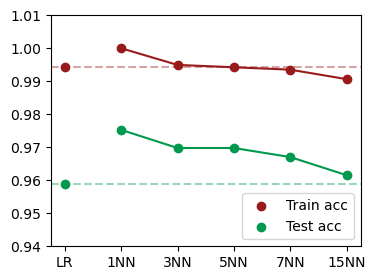
\includegraphics[width=0.4\textwidth]{Numerical/2.8.png}
	\caption{Accuracy as a function of the regressor. ``LR'' corresponds to Linear Regressor, and ``$i$NN'' corresponds to an $i$-nearest neighbors regressor.}
	\label{fig:Ex. 2.8}
\end{figure}

\textbf{Ex. 2.9: }Consider a linear regression model with $p$ parameters, fit by least squares to a set of training data $(x_1,y_1),\ldots,(x_N,y_N)$ drawn at random from a population. Let $\hat{\beta}$ be the least squares estimate. Suppose we have some test data $(\tilde{x}_1,\tilde{y}_1),\ldots,(\tilde{x}_M,\tilde{x}_M)$ drawn at random from the same population as the training data. If $R_{tr}(\beta)=\frac1N\sum_i^N\left(y_i-\beta^Tx_i\right)^2$ and $R_{te}(\beta)=\frac1M\sum_i^M\left(\tilde{y}_i-\beta^T\tilde{x}_i\right)^2$, prove that
\begin{align}
	\mathrm E[R_{tr}(\hat{\beta})]\leq\mathrm E[R_{ts}(\hat{\beta})],
\end{align}
where the expectations are over all that is random in each expression.

\textbf{Answer:}

Bear in mind that $\mathrm Ef(x_i,\,y_i,\,\hat{\beta})=\mathrm Ef(x_j,\,y_j,\,\hat{\beta})$. To see this, first note $\hat{\beta}$ is invariant with respect to changes of labels:
\begin{align}
	\hat{\beta}(\mathbf X,\,\mathbf y)&=\left(\mathbf X^T\mathbf X\right)^{-1}\mathbf X^T\mathbf y\\
	&=\left(\mathbf X^TS_{ij}^TS_{ij}\mathbf X\right)^{-1}\mathbf X^TS_{ij}^TS_{ij}\mathbf y\\
	&=\left(\left(S_{ij}\mathbf X\right)^T\left(S_{ij}\mathbf X\right)\right)^{-1}\left(S_{ij}\mathbf X\right)^T\left(S_{ij}\mathbf y\right)\\
	&=\hat{\beta}(S_{ij}\mathbf X,\,S_{ij}\mathbf y),
\end{align}
where $S_{ij}=S_{ij}^T=S_{ij}^{-1}$ is the $i$ to $j$ row operator. It then follows that
\begin{align}
	\mathrm Ef(x_i,\,y_i,\,\hat{\beta})&=\int P(\mathrm dx_1,\,\mathrm dy_1)\ldots P(\mathrm dx_N,\,\mathrm dy_N)\;f(x_i,\,y_i,\,\hat{\beta})\\
	&=\int P(\mathrm dx_1,\,\mathrm dy_1)\ldots P(\mathrm dx_N,\,\mathrm dy_N)\;f(x_j,\,y_j,\,\hat{\beta})\text{ }\left(\text{Change of labels}\right)\\
	&=\mathrm Ef(x_j,\,y_j,\,\hat{\beta}).
\end{align}

Thus,
\begin{align}
	\mathrm E[R_{tr}(\hat{\beta}(\mathbf X,\,\mathbf y))]&=\mathrm E\left[\frac1N\sum_i^N\left(y_i-\hat{\beta}^T(\mathbf X,\,\mathbf y)x_i\right)^2\right]\\
	&=\frac1N\sum_i^N\mathrm E\left(y_i-\hat{\beta}^T(\mathbf X,\,\mathbf y)x_i\right)^2\\
	&=\mathrm E\left(y_1-\hat{\beta}^T(\mathbf X,\,\mathbf y)x_1\right)^2,\\
	\mathrm E[R_{ts}(\hat{\beta}(\mathbf X,\,\mathbf y))]&=\mathrm E\left(\tilde{y}_1-\hat{\beta}^T(\mathbf X,\,\mathbf y)\tilde{x}_1\right)^2.
\end{align}

Now, for the comparison,
\begin{align}
	\mathrm E[R_{tr}(\hat{\beta}(\mathbf X,\,\mathbf y))]&=\mathrm E\left(y_1-\hat{\beta}^T(\mathbf X,\,\mathbf y)x_1\right)^2\\
	&=\mathrm Ey_1^2-2\mathrm Ey_1\hat{\beta}^T(\mathbf X,\,\mathbf y)x_1+\mathrm E\left[\hat{\beta}(\mathbf X,\,\mathbf y)^Tx_1\right]^2
\end{align}

Again I'm at a loss. It's time to move on.

\end{document}
\endinput
